% !TEX program = lualatex
\documentclass[10pt]{beamer}
\usepackage{luatexja}
\usepackage{amsmath}
\usepackage{amssymb}
\usepackage{amsthm}
\usepackage{bm}
\usepackage{eucal}
\usepackage{pdfpages}
\usepackage{tikz}
\usepackage{xcolor}
\usepackage{mathtools}

\renewcommand{\kanjifamilydefault}{\gtdefault}
\usetheme[block=fill]{metropolis}
\usefonttheme[onlymath]{serif}

\DeclareMathOperator{\diam}{diam}
\DeclareMathOperator{\id}{id}
\DeclareMathOperator{\Cay}{Cay}

\useinnertheme{rounded}
\setbeamertemplate{itemize items}[default]
\setbeamertemplate{enumerate items}[default]

\setbeamertemplate{theorems}[numbered]
% \makeatletter
% \@ifundefined{c@definition}{\newcounter{definition}}{}
% \makeatother

% \newtheorem{dfn}{Definition}[section]
% \newtheorem{prop}[dfn]{Proposition}
% \newtheorem{lem}[dfn]{Lemma}
% \newtheorem{thm}[dfn]{Theorem}
% \newtheorem{ex}[dfn]{Example}

\theoremstyle{definition}
\newtheorem{dfn}{Definition}[section]
\newtheorem{ex}[dfn]{Example}
\newtheorem{lem}[dfn]{Lemma}

\AtBeginEnvironment{dfn}{
    \setbeamercolor{block title}{fg=white, bg=blue!60!black}
    \setbeamercolor{block body}{bg=blue!5}
}

\AtBeginEnvironment{ex}{
    \setbeamercolor{block title}{fg=white, bg=green!50!black}
    \setbeamercolor{block body}{bg=green!5}
}

\AtBeginEnvironment{lem}{
    \setbeamercolor{block title}{fg=white, bg=orange!50!black}
    \setbeamercolor{block body}{bg=orange!5}
}

\title{テストスライド}
\author{おなまえ}
\date{\today}

\begin{document}
\begin{frame}
    \maketitle
\end{frame}

\begin{frame}
    \section{Cayley Graphs}
\end{frame}

\begin{frame}
    \frametitle{1}
    \begin{dfn}
    生成系 $S$ による群 $G$ の \textbf{Cayleyグラフ (Cayley graph)} とは
        \begin{enumerate}
            \item 頂点集合を $G$，
            \item 辺集合を $\{\{g,g\cdot s\}\mid g\in G，s\in(S\cup S^{-1})\setminus\{e\}\}$，
        \end{enumerate}
    とするグラフである．このグラフを $\Cay(G,S)$ と表記する．
    \end{dfn}

    \begin{ex}
        $\mathbb{Z}^2$ の生成系 $\{(1,0),(0,1)\}$ と，$\{(1,1),(0,1)\}$ に関するCayleyグラフは以下のようになる．
        \begin{figure}[h]
        \centering
        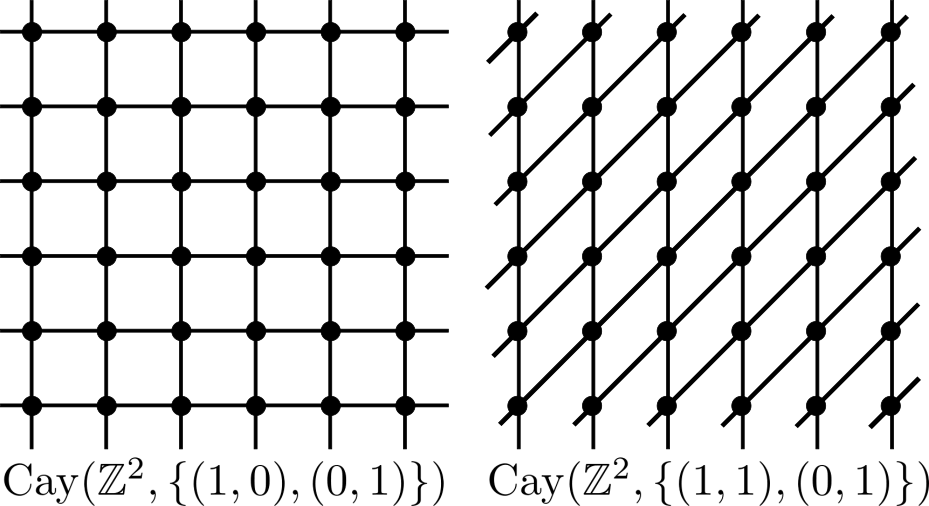
\includegraphics[width=48mm]{../picture/cayleyZ2_2.png}
        \end{figure}
    \end{ex}
\end{frame}

\begin{frame}
    \frametitle{2}
    \begin{dfn}
        生成系 $S$ による，群 $G$ 上の \textbf{word metric} とは，$d_S\colon G\times G\rightarrow \mathbb{N}_{\geq 0}$，
        \begin{equation*}
            d_S(g,h)\coloneqq\min\{n\in\mathbb{N}_{\geq 0}\mid s_1,s_2,\ldots, s_n\in S\cup S^{-1}，g^{-1}h=s_1s_2\cdots s_n\}
        \end{equation*}
        であり，これは $G$ 上の距離関数である．
    \end{dfn}
    この距離関数は，$\Cay(G,S)$の一辺の長さを1としてえられる距離関数と同じである．また，この距離関数は生成系に依存する．\\

    この関数により，$(G,d_S)$ は距離空間となる．
\end{frame}

\begin{frame}
    \section{Quasi-isometries}
\end{frame}

\begin{frame}
    \frametitle{3}
    以下，$(X,d_X)$ を距離空間とし，省略して $X$ と表記する．
    \begin{dfn}
        写像 $f\colon X\rightarrow Y$ が \textbf{等長埋め込み (isometric embedding)} であるとは，任意の $x,x^\prime\in X$ に関して，$$d_X(x,x^\prime)=d_Y(f(x),f(x^\prime))$$ が成り立つことをいう．また，$f$ が \textbf{等長写像 (isometry)} であるとは，以下の二条件を満たすときをいう．
        \begin{enumerate}
        \item $f$ が等長埋め込みである．
        \item ある等長埋め込み $g\colon Y\rightarrow X$ が存在し，$f\circ g=\id_Y，g\circ f=\id_X$ を満たす．
        \end{enumerate}
        さらに，二つの距離空間 $X,Y$ が \textbf{等長 (isometric)} であるとは，等長写像 $f\colon X\rightarrow Y$ が存在するときをいう． 
    \end{dfn}
\end{frame}

\begin{frame}
    \frametitle{4}
    \begin{dfn}
        写像 $f\colon X\rightarrow Y$ が \textbf{bilipschitz埋め込み (bilipschitz embedding)} であるとは，ある定数 $c\in\mathbb{R}_{>0}$ が存在し，任意の $x,x^\prime\in X$ に対して，
        $$\frac{1}{c}d_X(x,x^\prime)\leq d_Y(f(x),f(x^\prime))\leq cd_X(x,x^\prime)$$
        が成り立つことをいう．また，$f$ が \textbf{bilipschitz equivalence (bi-Lip)} であるとは，以下の二条件を満たすときをいう．
        \begin{enumerate}
        \item $f$ がbilipschitz埋め込みである．
        \item あるbilipschitz埋め込み $g\colon Y\rightarrow X$ が存在し，$f\circ g=\id_Y$，$g\circ f=\id_X$ を満たす．
        \end{enumerate}
        さらに，二つの距離空間 $X,Y$ が \textbf{bilipschitz equivalent} であるとは，bilipschitz equivalence な写像 $f\colon X\rightarrow Y$ が存在するときをいう．
    \end{dfn}
\end{frame}

\begin{frame}
    \frametitle{5}
    \begin{ex}
        通常の距離が入った距離空間 $\mathbb{Z},2\mathbb{Z}$ に対し， $f\colon\mathbb{Z}\rightarrow 2\mathbb{Z}$ を，$f(n)=2n$ とすると，これは等長埋め込みではないが bilipschitz埋め込みであるまた，$g\colon2\mathbb{Z}\rightarrow \mathbb{Z}$ を，$g(m)=m/2$ とすれば，$f,g$ によって $\mathbb{Z}$ と $2\mathbb{Z}$ は bilipschitz equivalent である．
    \end{ex}
    \begin{dfn}
        写像 $f\colon X\rightarrow Y$ が 写像 $f^\prime\colon X\rightarrow Y$ から\textbf{finite distance} であるとは，ある定数$c\in\mathbb{R}_{>0}$ が存在し，任意の $x\in X$ に対して，
        $$d_Y(f(x),f^\prime(x))\leq c$$
が成り立つことをいう．
    \end{dfn}
\end{frame}

\begin{frame}
    \frametitle{6}
    \begin{dfn}
        写像 $f\colon X\rightarrow Y$ が \textbf{擬等長埋め込み (quasi-isometric embedding)} であるとは，ある定数 $c\in\mathbb{R}_{>0}$，$b\in\mathbb{R}_{\geq0}$ が存在し，任意の $x,x^\prime\in X$ に対して，
        $$\frac{1}{c}d_X(x,x^\prime)-b\leq d_Y(f(x),f(x^\prime))\leq cd_X(x,x^\prime)+b$$
        が成り立つことをいう．このとき，$f$ を \bm{$(c,b)$}\textbf{-quasi-isometric embedding} とも表現する．また，$f$ が\textbf{擬等長写像 (quasi-isometry, QI)} であるとは，以下の二条件を満たすときをいう．
        \begin{enumerate}
        \item $f$ が擬等長埋め込みである．
        \item ある擬等長埋め込み $g\colon Y\rightarrow X$ が存在し，
        $f\circ g$ が $\id_Y$ から finite distance，$g\circ f$ が $\id_X$ から finite distance である．
        \end{enumerate}
        さらに，二つの距離空間 $X,Y$ が \textbf{擬等長 (quasi-isometric)} であるとは，擬等長写像 $f\colon X\rightarrow Y$ が存在するときをいう．
    \end{dfn}
\end{frame}

\begin{frame}
    \frametitle{7}
    \begin{ex}
        通常の距離が入った距離空間 $\mathbb{R},\mathbb{Z}$ に対し， $f\colon\mathbb{R}\rightarrow\mathbb{Z}$ を，$f(x)=\lfloor x \rfloor$ と定めると，これは bilipschitz embedding ではないが，擬等長埋め込みである．また，$\mathbb{Z}$ から $\mathbb{R}$ への包含写像を考えると，$f$ と包含写像によって $\mathbb{Z}$ と $\mathbb{R}$ は擬等長である．
    \end{ex}

    擬等長埋め込みは連続とは限らない(実際上の例の $f$ は連続でない)．同様に，擬等長写像は連続であるとは限らない．
    \begin{figure}[h]
    \centering
    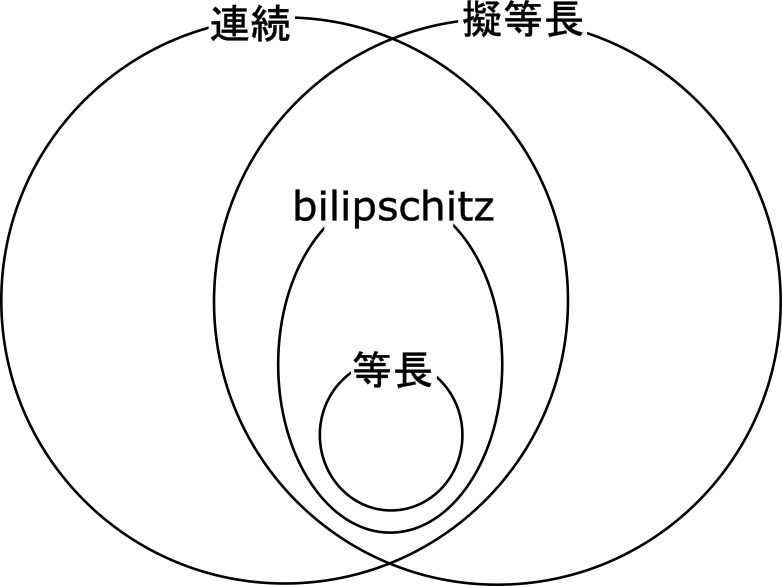
\includegraphics[width=55mm]{../picture/benzu}
    \label{map}
    \end{figure}
\end{frame}

\begin{frame}
    \frametitle{8}
    \begin{dfn}
        $G$ を有限生成群としたとき，$G$ が距離空間 $X$ に \textbf{bilipschitz equivalent} であるとは，$G$ のある有限な生成系 $S$ がとれ，距離空間 $(G,d_S)$ と $X$ が (先ほど定義した) bilipschitz equivalent であることをいう．\\
        
        また，$G$ が $X$ に \textbf{擬等長 (quasi-isometric)} であるとは，ある有限な生成系 $S$ がとれ，距離空間 $(G,d_S)$ と $X$ が (先ほど定義した) quasi-isometric であることをいう．
    \end{dfn}
    群 $G$ の生成系 $S$ が有限であることに注意．

\end{frame}

\section{Quasi-Geodesic Metric Spaces}

\begin{frame}
    \frametitle{9}
    \begin{dfn}
    距離空間 $X$ 上の長さ $L\in\mathbb{R}_{>0}$ の \textbf{測地線 (geodesic)} とは，$[0,L]\subset\mathbb{R}$ から $X$ への等長埋め込み，つまり任意の二点 $t_1,t_2\in [0,L]$ に対し，
    $$|t_2-t_1|=d_X(\gamma(t_2),\gamma(t_1))$$
    をみたす $\gamma\colon[0,L]\rightarrow X$ のことである．

    また，$X$ が \textbf{測地的 (geodesic)} であるとは，任意の $x,x^\prime\in X$ において，$\gamma(0)=x$，$\gamma(L)=x^\prime$ となるような 等長埋め込み $\gamma$ がとれるときをいう．
    \end{dfn}

    \begin{ex}
        通常の距離が入った $\mathbb{R}^n$ は測地的だが，$\mathbb{R}^n\setminus\{0\}$ は測地的でない．実際，$(1,0)$ と $(-1,0)$ 間の距離は $2$ だが，この測地線は原点を通ってしまう．
    \end{ex}
\end{frame}

\begin{frame}
    \frametitle{10}
    \begin{dfn}
    距離空間 $X$ 上の \textbf{\bm{$(c,b)$}-擬測地線 (\bm{$(c,b)$}-quasi-godesic)} とは，$[0,L]\subset\mathbb{R}$ から $X$ への $(c,b)$-擬等長埋め込み，つまり任意の二点 $t_1,t_2\in [0,L]$ に対し，
    $$\frac{1}{c}|t_2-t_1|-b\leq d_X(\gamma(t_2),\gamma(t_1))\leq c|t_2-t_1|+b$$
    をみたす $\gamma\colon[0,L]\rightarrow X$ のことである．
    
    また，$X$ が \textbf{\bm{$(c,b)$}-擬測地的 (\bm{$(c,b)$}-quasi-godesic)} であるとは，任意の $x,x^\prime\in X$ において，$\gamma(0)=x$，$\gamma(L)=x^\prime$ となるような $(c,b)$-擬等長埋め込み，$\gamma$ がとれるときをいう(単に擬測地線や擬測地的ともいう)．
    \end{dfn}

    \begin{ex}
    通常の距離が入った $\mathbb{R}^n\setminus\{0\}$ は，$(1,\epsilon)$-測地的である($\epsilon>0$)．これは，原点中心で十分小さい半径の円で原点を迂回すれば，擬測地線が得られるからである．
    \end{ex}
\end{frame}

\section{Švarc-Milnor Lemma}

\begin{frame}
    \frametitle{11}
    \begin{lem}[Švarc-Milnor Lemma]
        $G$ を群とし，$(c,b)$-測地的な距離空間 $(X,d_X)$ 上に等長な群作用があるとする ($b,c>0$)．もしある部分集合 $B\subset X$ が存在し，
    \begin{enumerate}
    \item[(a)] $\diam B\coloneqq\underset{x,y\in B}{\sup}d(x,y)<\infty,$
    \item[(b)] $\bigcup_{g\in G}g\cdot B=X,$
    \item[(c)] 集合 $S\coloneqq\{g\in G\mid g\cdot B^\prime \cap B^\prime \neq \emptyset\}$ が有限
    \end{enumerate}
    を満たすならば，
    \begin{enumerate}
    \item $S$ は $G$ の有限生成系であり，\label{S_is_generating_set}
    \item 任意の $x\in X$ に対して定まる写像 $\varphi\colon G\rightarrow X\;;\; g\mapsto g\cdot x$ によって，$G$ と $X$ は擬等長である．\label{G~X}
    \end{enumerate}
    ただし，$B^\prime \coloneqq\{x\in X\mid y\in B，d_X(x,y)\leq 2b\}$ と定める．
    \end{lem}
\end{frame}

\end{document}